\documentclass{standalone}
\usepackage{tikz}
\usepackage{pgfplots}
\usepackage{xparse}
\pgfplotsset{compat=1.12,width=7cm}%
\colorlet{curveZero}{gray!85}
\colorlet{curveOne}{blue!60}
\definecolor{curveOneColor}{rgb}{.6,0,0}
\colorlet{curveTwo}{brown!50!gray}
\colorlet{curveThree}{green!40!gray}
\colorlet{curveFour}{red!50!gray}
\NewDocumentCommand\DrawDotInPlot{O{}mmO{}}%
{%
\fill[gray!15,draw=gray] (axis cs:{#2},{#3}) circle [radius=1.6pt] node[above,black,#4] {\(#1\)};%
}%
\NewDocumentCommand\DrawDot{O{}mmO{}}%
{%
\fill[gray!20,draw=gray] ({#2},{#3}) circle (1.6pt) node[above,black,#4] {\(#1\)};%
}%
\NewDocumentCommand\DrawNode{O{}m}%
{%
\fill[gray!20,draw=gray] (#2) circle (1.6pt) node[above,black] {\(#1\)};%
}%
\NewDocumentCommand\DrawDotThreeD{O{}mmmO{}}%
{%
\fill[gray!20,draw=gray] ({#2},{#3},{#4}) circle (1.6pt) node[above,black,#5] {\(#1\)};%
}%
\colorlet{axisColor}{gray!50}
\tikzstyle{shapeZero}=[fill=curveZero,opacity=.4]
\tikzstyle{shapeOne}=[fill=curveOne,opacity=.4]
\tikzstyle{shapeTwo}=[fill=curveTwo,opacity=.4]
\tikzstyle{shapeThree}=[fill=curveThree,opacity=.4]
\tikzstyle{groupElementLabel}=[minimum size=2.4em]
\tikzstyle{groupElement}=[minimum size=2.4em,shapeZero,draw=curveZero]
\tikzstyle{cosetOne}=[minimum size=2.4em,shapeOne,draw=curveOne]
\tikzstyle{cosetTwo}=[minimum size=2.4em,shapeTwo,draw=curveTwo]


\begin{document}
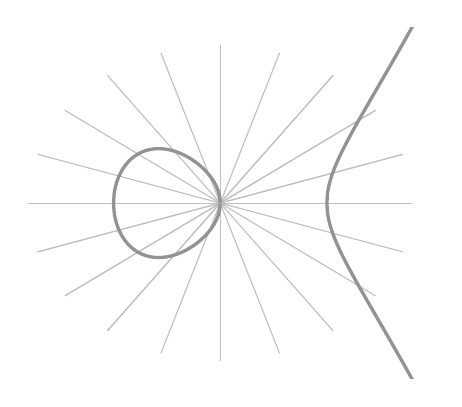
\begin{tikzpicture}
\begin{axis}[hide axis,xmin=-2,xmax=2,ymin=-2,ymax=2]
\newcommand{\RRR}{1.8}
\draw[axisColor] 
	({\RRR*cos(3.1415*0/10 r)},{\RRR*sin(3.1415*0/10 r)}) 
-- ({-\RRR*cos(3.1415*0/10 r)},{-\RRR*sin(3.1415*0/10 r)});
\draw[axisColor] 
	({\RRR*cos(3.1415*1/10 r)},{\RRR*sin(3.1415*1/10 r)}) 
-- ({-\RRR*cos(3.1415*1/10 r)},{-\RRR*sin(3.1415*1/10 r)});
\draw[axisColor] 
	({\RRR*cos(3.1415*2/10 r)},{\RRR*sin(3.1415*2/10 r)}) 
-- ({-\RRR*cos(3.1415*2/10 r)},{-\RRR*sin(3.1415*2/10 r)});
\draw[axisColor] 
	({\RRR*cos(3.1415*3/10 r)},{\RRR*sin(3.1415*3/10 r)}) 
-- ({-\RRR*cos(3.1415*3/10 r)},{-\RRR*sin(3.1415*3/10 r)});
\draw[axisColor] 
	({\RRR*cos(3.1415*4/10 r)},{\RRR*sin(3.1415*4/10 r)}) 
-- ({-\RRR*cos(3.1415*4/10 r)},{-\RRR*sin(3.1415*4/10 r)});
\draw[axisColor] 
	({\RRR*cos(3.1415*1/10 r)},{-\RRR*sin(3.1415*1/10 r)}) 
-- ({-\RRR*cos(3.1415*1/10 r)},{\RRR*sin(3.1415*1/10 r)});
\draw[axisColor] 
	({\RRR*cos(3.1415*2/10 r)},{-\RRR*sin(3.1415*2/10 r)}) 
-- ({-\RRR*cos(3.1415*2/10 r)},{\RRR*sin(3.1415*2/10 r)});
\draw[axisColor] 
	({\RRR*cos(3.1415*3/10 r)},{-\RRR*sin(3.1415*3/10 r)}) 
-- ({-\RRR*cos(3.1415*3/10 r)},{\RRR*sin(3.1415*3/10 r)});
\draw[axisColor] 
	({\RRR*cos(3.1415*4/10 r)},{-\RRR*sin(3.1415*4/10 r)}) 
-- ({-\RRR*cos(3.1415*4/10 r)},{\RRR*sin(3.1415*4/10 r)});
\draw[axisColor] 
	({\RRR*cos(3.1415*1/10 r)},{\RRR*sin(3.1415*1/10 r)}) 
-- ({-\RRR*cos(3.1415*1/10 r)},{-\RRR*sin(3.1415*1/10 r)});
\draw[axisColor] 
	({\RRR*cos(3.1415*2/10 r)},{\RRR*sin(3.1415*2/10 r)}) 
-- ({-\RRR*cos(3.1415*2/10 r)},{-\RRR*sin(3.1415*2/10 r)});
\draw[axisColor] 
	({\RRR*cos(3.1415*3/10 r)},{\RRR*sin(3.1415*3/10 r)}) 
-- ({-\RRR*cos(3.1415*3/10 r)},{-\RRR*sin(3.1415*3/10 r)});
\draw[axisColor] 
	(0,\RRR) 
-- (0,{-\RRR});
\addplot[very thick,domain=-1:0,curveZero,samples=200]{sqrt((x+1)*x*(x-1))};%
\addplot[very thick,domain=-1:0,curveZero,samples=200]{-sqrt((x+1)*x*(x-1)))};%
\addplot[very thick,domain=1:2,curveZero,samples=200]{sqrt((x+1)*x*(x-1)))};%
\addplot[very thick,domain=1:2,curveZero,samples=200]{-sqrt((x+1)*x*(x-1)))};%
\DrawDotInPlot{0}{0}
%\fill[gray!20,draw=gray] (axis cs:0,0) circle (1.3pt);
\end{axis}
\end{tikzpicture}
\end{document}
